
During this week, we will work on the digital design that is running on the LimeSDR FPGA. We will make modifications to the design and compile it using Quartus. The Lime Suite GUI tool is then needed to flash the design on the FPGA. Below, you will find the instructions for the installation and configuration of the tools employed.\\

\section{Installing Quartus Prime Lite and the device support package}

Most of you probably follow the course LELEC2531 for which you have installed Quartus Prime Lite 18.1. If you have already  it installed, you can skip this paragraph. To install Quartus, follow this link~: \href{https://www.intel.com/content/www/us/en/products/details/fpga/development-tools/quartus-prime/resource.html}{Quartus Website}. Then click on the \textit{Quartus Prime Lite} version for you OS, select the 18.1 version and follow the download and install instructions.\\

If you already have Quartus installed, you might not have the required device support package for the MAX 10 device family that we use in this project. You can download the package \href{https://www.intel.com/content/www/us/en/products/details/fpga/development-tools/quartus-prime/resource.html}{here} by first clicking on your Quartus installation, most probably the Prime Lite. Then select the Quartus version installed on your computer.
Under the download section, go in the \textit{"Individual Files"} and download the \textit{"Intel® MAX® 10 Device Support"}. On your computer, launch the \textit{"Device Installer (Quartus Prime)"} from the start menu. If you cannot find it, it should be located in your Quartus installation folder at \texttt{"intelFPGA/18.1/quartus/common/devinfo/dev\_install"}.
The programm will ask you to select the folder in which the downloaded file is located, it will then automatically detect the MAX 10 device support file. You can proceed to the installation.

\section{Installing the LimeSuite components}

The Lime Suite GUI tool is needed to flash your FPGA. This program is already preinstalled on the virtual machine we provided you. Quartus is installed on your host system, meaning that you have to transfer the compiled design from your host system to the virtual machine when you want to flash the FPGA with a new design. You can do so via a USB flash drive, via Internet, by using a shared folder between your host and guest system, or by installing LimeSuite on your host system. As the latter can be tricky, we recommend you to use a shared folder to transfer the compiled file from Quartus to the VM.

\subsection{(Recommended) Shared folder between host system and VM}

Setting up the shared folder features requires to first install the \textit{Guest Additions}. To do so, start the VM and then go to Devices (top of the VirtualBox window) and click on \textit{Insert Guest Additions CD image...}. A new device will be plugged in the VM. You can access it by opening a terminal, going into the media folder and running VBoxLinuxAdditions.run (with admin rights).
\begin{figure}[H]
    \centering
    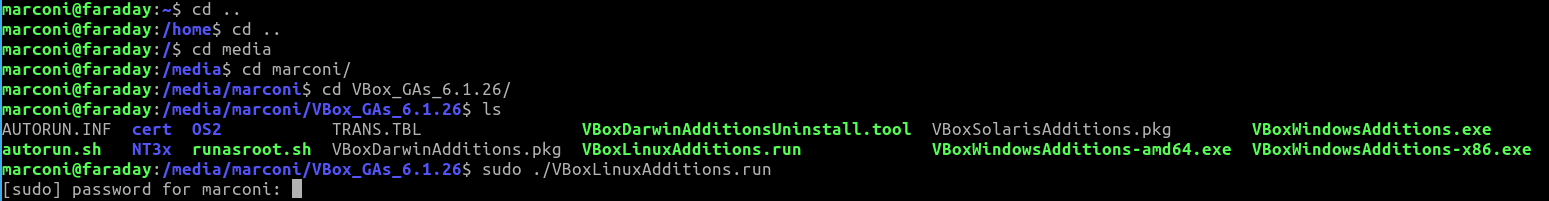
\includegraphics[width=0.95\textwidth]{figures/run_VBOX.PNG}
	\caption{How to run VBoxLinuxAdditions.}
	\label{figrun}
\end{figure}
After the run is complete, you need to restart the VM. Next you need to enable the shared folder feature and to actually create this virtual bridge between the host system and the VM.

\begin{enumerate}
    \item In the VM, click on the Devices menu and then \textit{Shared Folders>Shared Folder Settings}.
    \item In this settings menu, click the blue icon to add a new shared folder. Select the folder path drop-down and choose other. Choose the folder you want to share and click \textit{Select Folder}.
    \begin{figure}[H]
    \centering
    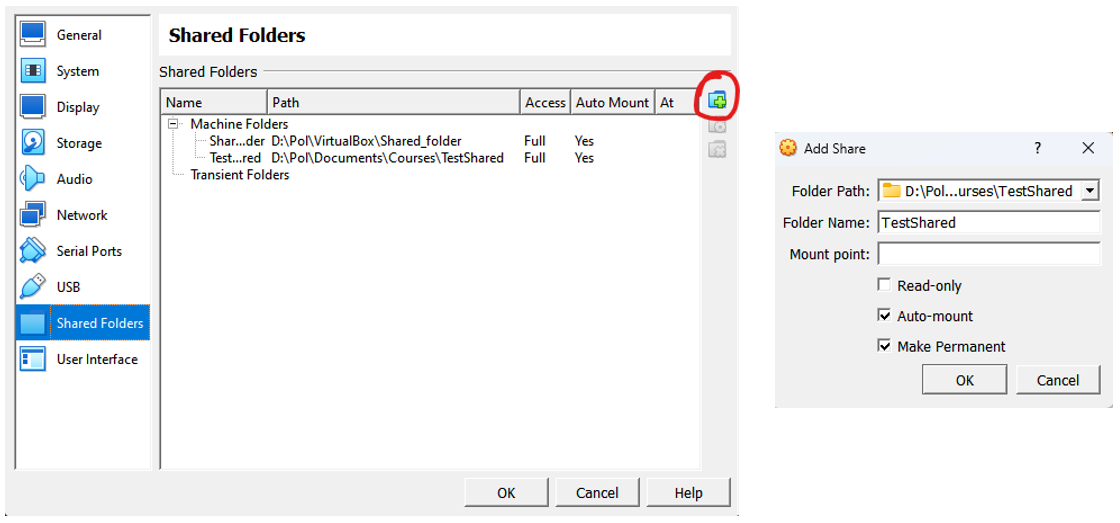
\includegraphics[width = \textwidth]{figures/settings_shared_folder_full.png}
	\caption{How to add a new shared folder.}
	\label{figrun}
    \end{figure}
    \item Select auto-mount and then click OK two times. Be careful, if you close the Settings window without pressing OK, your modifications will not be applied.
\end{enumerate}




\subsection{Install LimeSuite on your host system}

The instructions are provided for the different OS on the \href{http://wiki.myriadrf.org/Lime_Suite}{Myriad-RF Wiki}. The LimeSDR-Mini might not be recognized by your host system and additional drivers should then be installed. Please follow the instructions provided \href{https://wiki.myriadrf.org/LimeSDR_Windows_Driver_Installation}{here}.




\section{Testing LimeSuite}

Disregarding the way you use LimeSuite (on host guest or in the VM), you need to test that you can flash the FPGA. To do so, open the Lime Suite GUI tool and connect the LimeSDR. Do not forget to make the USB passthrough if you use the LimeSuite on the VM. We will perform a flash of the default design. To this end, go to \textit{Options -> Connection Settings} and connect to the device. You should observe in the console that the LimeSDR Mini board is now correctly connected. Then, open the programming panel in \textit{Modules -> Programming}, select the \textit{Automatic} mode and launch the flashing using the \textit{Program} button.

\subsection{Possible issues}
The LimeSDR-Mini can crash and prompt errors during programming which might be linked to the USB driver version. Here are some hints.

\subsubsection{LimeSuite on host system}
You might have USB3.0 drivers installed on your computer. However, the USB extension cable might interfere and show the LimeSDR as an USB2.0 in LimeSuite. A work-around is to flash the LimeSDR without using the USB extension cable. Do not forget to replug it afterward, this trick should only be applied for programming purposes.


\subsubsection{LimeSuite on Virtual Machine}
As for now, LimeSuite on the VM seems to prefer flashing via an USB2.0 interface. If the programming does not work in your current configuration, look in the USB tab of the VM settings. There, select USB 2.0 or lower, as we have encountered issues with USB 3.0.
